% command to make sure colorboxes don't create whitespace between code lines
\fboxsep=.6pt

% default settings for listings
\lstset{style=python}

\title[Programmieren]{Programmieren: Datenstrukturen}

\subtitle{Listen Verändern}

\author[Blum, Cyril] % (optional)
{Cyril Blum}

\institute[KLW] % (optional)
{
	Fachschaft Informatik\\
	Kantonsschule im Lee
}

\date[\today] % (optional)

\logo{
\includegraphics[width=2cm]{Logos/FreeFlower.pdf}}

\titlegraphic{\vspace{-.7cm}\includegraphics[width=\textwidth]{"Grundlagen_Info/06_Datenbanken/Figures/title-emojis"}}

\frame{\titlepage}

\begin{frame}[fragile]{Beispiel: Tram}
Sie leiten die Entwicklung des Tram-Fahrplans in der Stadt Zürich. Die aktuelle Glatttalbahn (Tram 12) fährt von Stettbach, bzw. Oerlikon, bis zum Flughafen (siehe folgende Abbildungen). Ignorieren Sie die blaue Linie, die bei \enquote{Glattpark} nach rechts abbiegt.
\end{frame}
\begin{frame}[fragile]{Beispiel: Tram}

\begin{figure}[H]
\centering
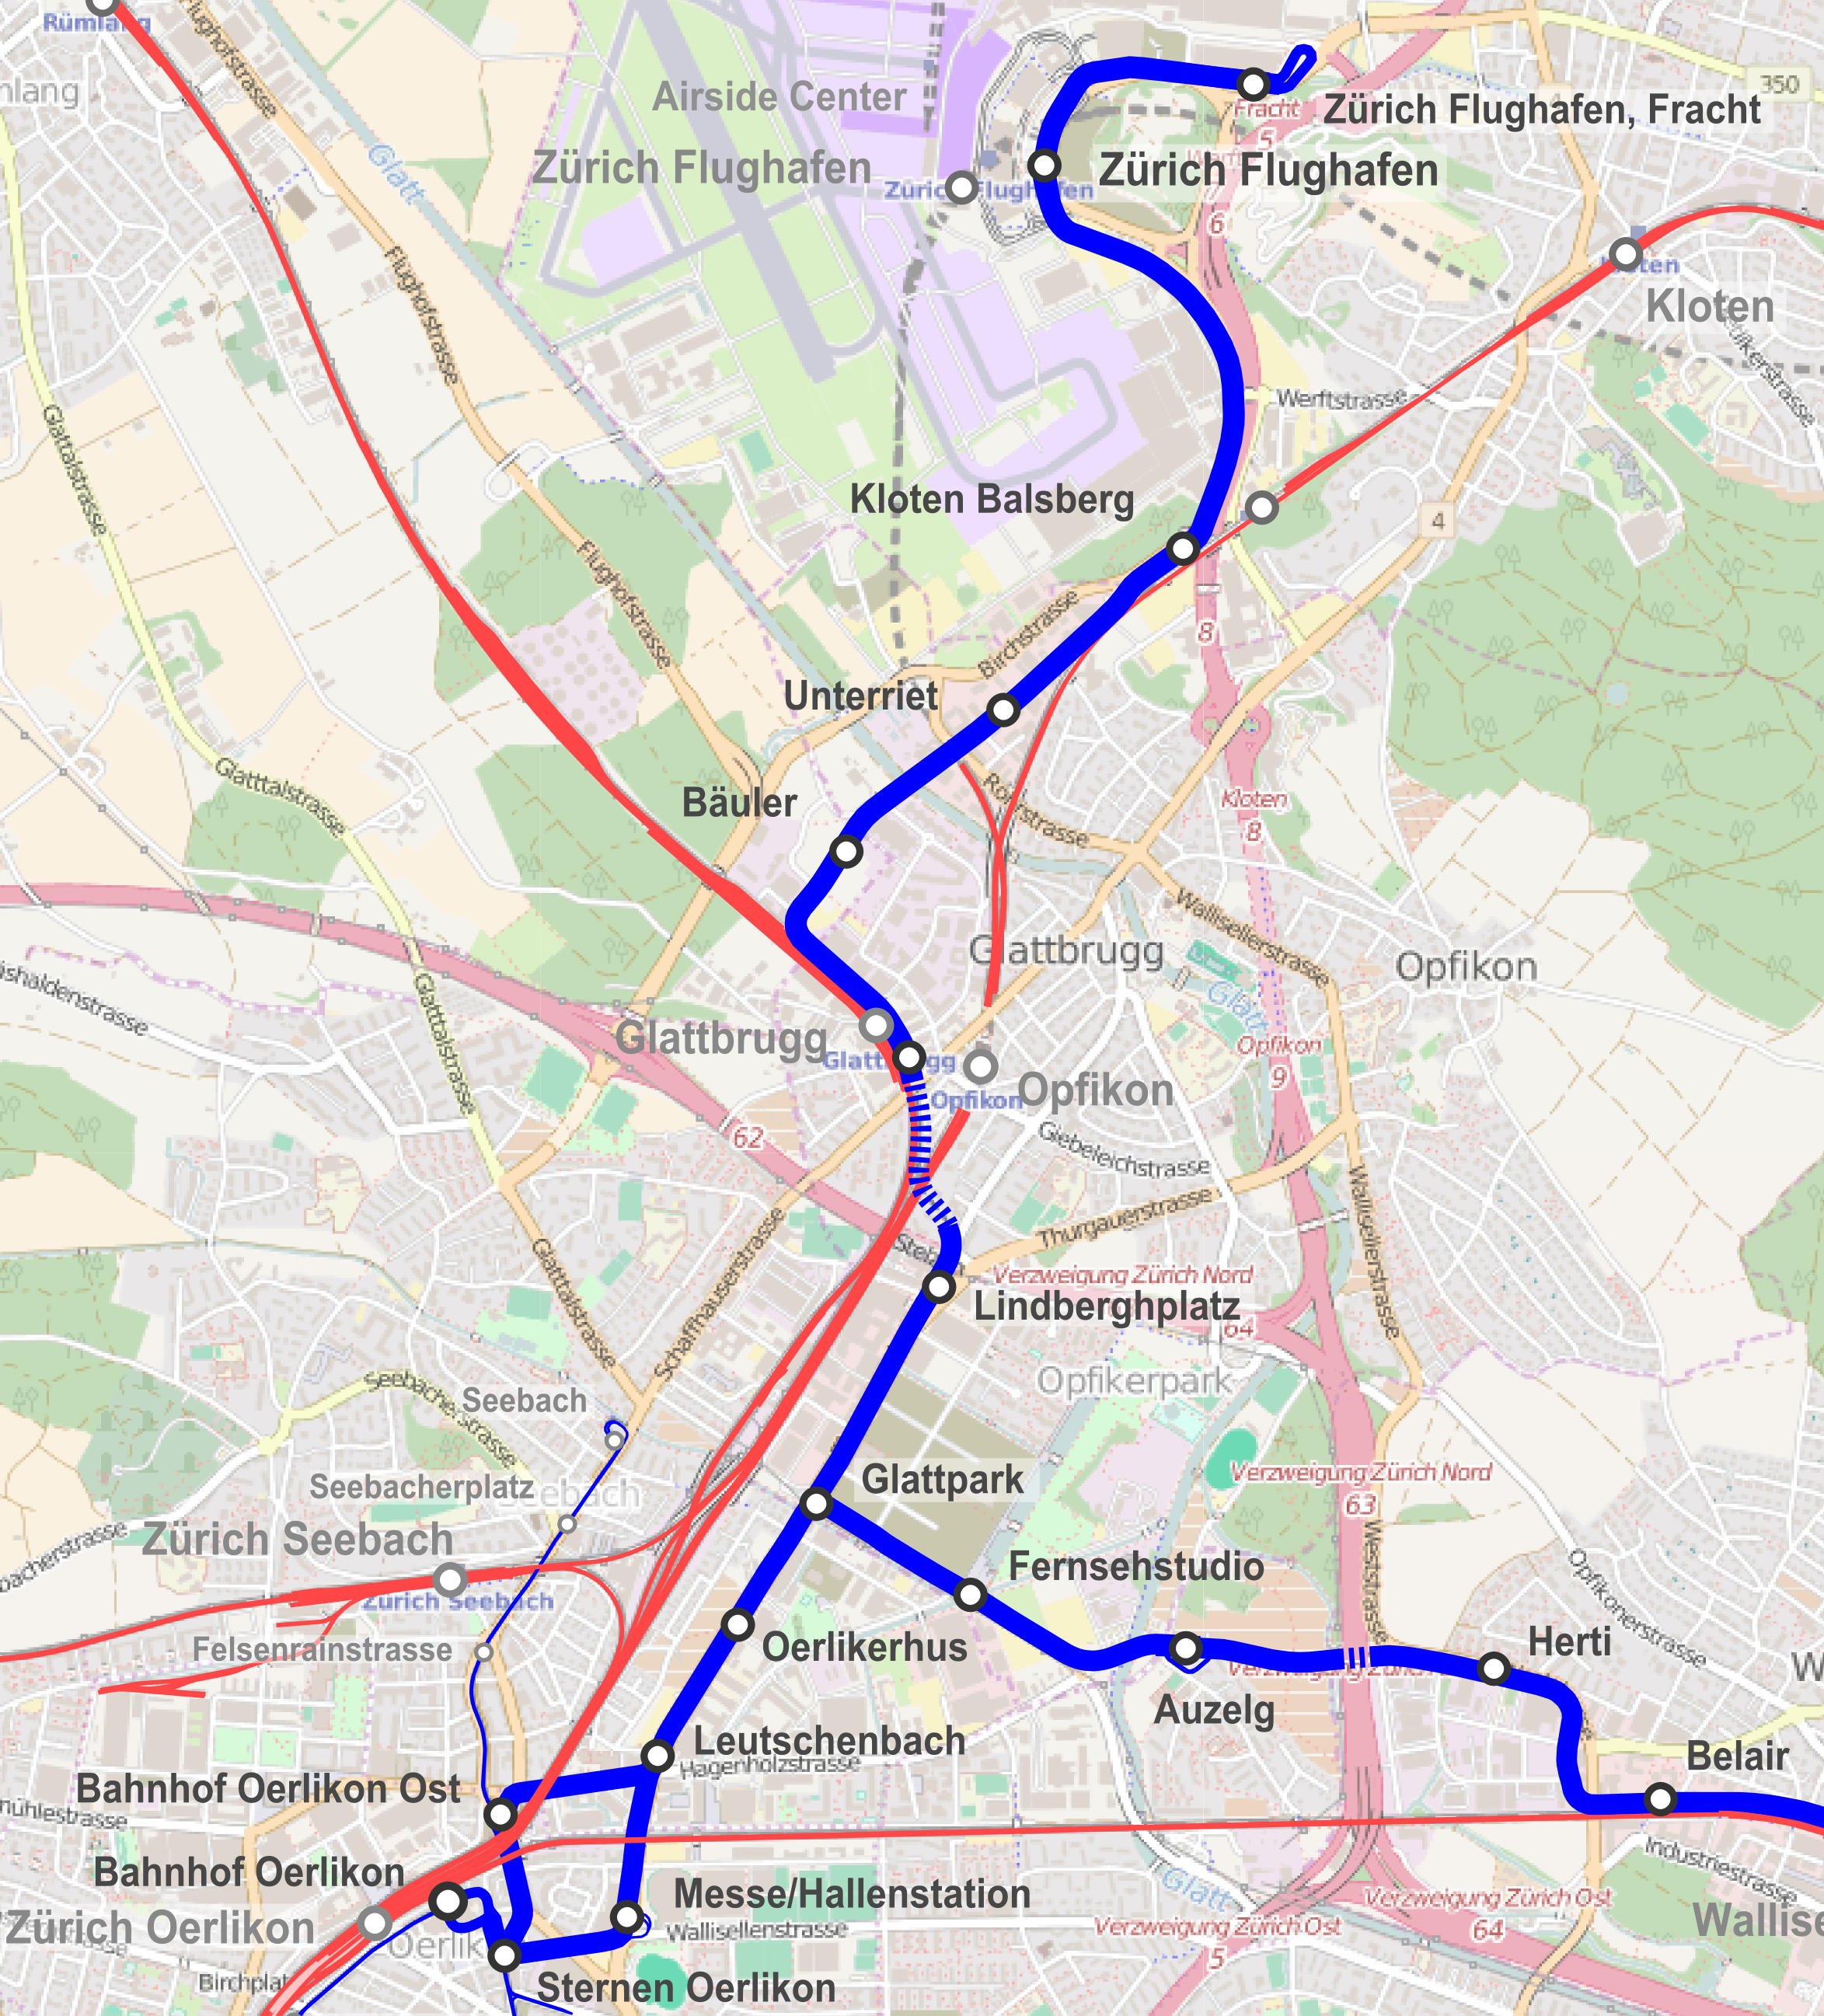
\includegraphics[width=.6\linewidth]{Grundlagen_Info/00_Programmieren/Figures/Glattalbahn_vbg}
\end{figure}

\end{frame}
\begin{frame}[fragile]{Beispiel: Tram}

Sie haben sich folgende Stationen und die Fahrzeit von der Anfangs-Station \enquote{Sternen Oerlikon} zu jeder folgenden Station bis und mit \enquote{Zürich Flughafen Fracht} in Sekunden notiert:

\begin{lstlisting}
stationen = ["Sternen", "Messe", "Leutschenbach", "Oerlikerhus", "Glattpark", "Lindbergh", "Glattbrugg", "Bäuler", "Unterriet", "Kloten", "Flughafen", "Flughafen Fracht"]
dauer = [0, 60, 122, 185, 241, 363, 543, 603, 666, 729, 786, 845]
\end{lstlisting}

Die Glattal-Tramlinie soll nun erweitert werden um die folgenden Stationen:
\end{frame}

\begin{frame}[fragile]{Beispiel: Tram}
\begin{figure}
\centering
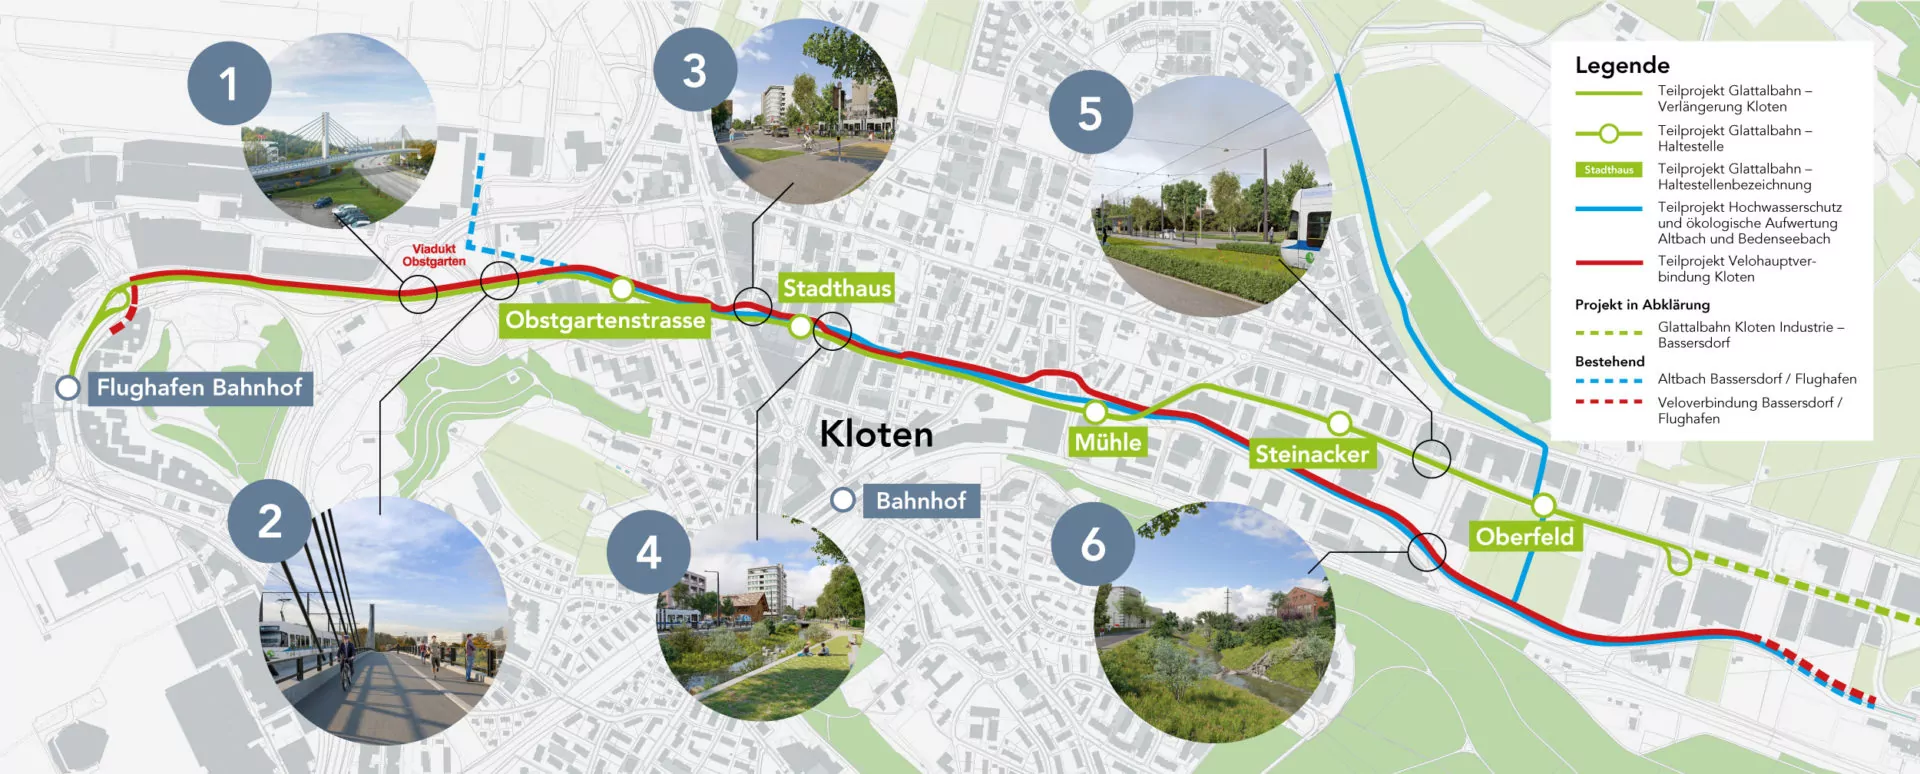
\includegraphics[width=\linewidth]{Grundlagen_Info/00_Programmieren/Figures/GTB_Karte_mit_Legende_Web_v02}
\end{figure}
Was könnten wir im Code ändern, falls wir die Liste erweitern wollen?
\end{frame}
    


\begin{frame}[fragile]{Datenstrukturen: Stapel \emoji{books}}
	\begin{itemize}
		\item \lstinline|meineliste.append(neu)|: Fügt ein Element \lstinline|neu| (einzelne Zahl oder Text) am Ende der Liste \lstinline|meineliste| hinzu
		\item \lstinline|meineliste.pop()|: Entfernt das letzte Element von \lstinline|meineliste|
		\item \lstinline|meineliste.pop(2)|: Entfernt das Element an dritter Stelle von \lstinline|meineliste| 
	\end{itemize}
	\pause
	Beispiel:
	\begin{lstlisting}
	# stationen von vorher
	stationen = ["Sternen", "Messe", "Leutschenbach", "Oerlikerhus", "Glattpark", "Lindbergh", "Glattbrugg", "Bäuler", "Unterriet", "Kloten", "Flughafen", "Flughafen Fracht"]
	
	stationen.append("Obstgartenstrasse")
	stationen.append("Stadthaus")
	#...	
	\end{lstlisting}
\end{frame}

\begin{frame}[fragile]{Beispiel}
	\begin{lstlisting}[numbers=left,escapechar=|]
		zahlen = [-12, 5, 6, 9]
		weitere_zahl = 22
		zahlen.append(weitere_zahl)
		print(zahlen) # |\only<1>{\textcolor{blue}{Was wird gedruckt?}}||\only<2->{\textcolor{blue}{[-12, 5, 6, 9, 22]}}|

		zahlen.pop()
		zahlen.pop()
		print(zahlen) # |\only<1-2>{\textcolor{blue}{Was wird gedruckt?}}||\only<3->{\textcolor{blue}{[-12, 5, 6]}}|
	\end{lstlisting}
\end{frame}

\begin{frame}[fragile]{Auf Listen zugreifen}{Von hinten}
Gegeben sei folgende Liste: \lstinline|x=[3, 10, 33, 2, 220, 11]|.\\

Wie können wir auf das letzte Element von \lstinline|x| (= die Zahl \lstinline|11|) zugreifen?
\begin{itemize}
\item \lstinline|x[len(x)-1]|
\item Einfacher: \lstinline|x[-1]|
\item Vorletztes Element: \lstinline|x[-2]|
\item Etc.
\end{itemize}
\end{frame}

\begin{frame}[fragile]{Fibonacci-Serie}
\begin{itemize}[<+->]
\item Was ist die Fortsetzung folgender Zahlen? 1, 1, 2, 3, 5, ...?
\item Wie würden wir einen Code dafür schreiben?
	\begin{lstlisting}
fib = [1, 1]
for _ in range(100):
	# berechne nächste Zahl
	fib_neu = fib[-1] + fib[-2]
	fib.append(fib_neu)
print(fib)
	\end{lstlisting}
\end{itemize}
\def\spiral#1{%
  \pgfmathparse{int(#1)}%
  \ifnum\pgfmathresult>0
    \draw [help lines] (0,0) rectangle ++(1,1);
    \begin{scope}[shift={(1,1)}, rotate=90, scale=1/1.6180339887]
      \spiral{#1-1}
    \end{scope}
    \draw [red] (0,0) arc (270:360:1);
  \fi
}

\begin{figure}[H]
\centering
\tikz[scale=2]{\spiral{12}}
\end{figure}
\end{frame}



\begin{frame}[fragile]{Auftrag}{Skript, Abschnitt 6.1.3}
	\begin{itemize}
		\item \readbox{Definition 6.2, Beispiel 6.9}
		\item \aufgabebox{Aufgaben 6.15-6.19}
		\item \challengebox{Aufgabe 6.20}
		\item Lernkontrolle auf Moodle (Dynamische Datenstrukturen)
	\end{itemize}
\end{frame}




% \begin{frame}[fragile]{Appendix: Überprüfen, ob etwas in einer Liste ist}{Mani Matter (\href{https://youtu.be/gQbF9Ck1ccc?feature=shared}{Link})}
	
% 	\begin{lstlisting}
% 		zutaten_sandwich = ["brot", "fleisch", "anke", "brot"]
		
% 		if "brot" not in zutaten_sandwich:
% 			print("Was isch es Sandwich ohni Brot? S'isch nume Fleisch!")
% 		elif "fleisch" not in zutaten_sandwich:
% 			print("Was isch es Sandwich ohni Fleisch? S'isch nume Brot!")
% 		# usw. 
% 	\end{lstlisting}
% \end{frame}

% \begin{frame}[fragile]{Appendix: Überprüfen, an welcher Position in einer Liste ein Element ist}
	
% \begin{lstlisting}
% stationen = ["Bern", "Zürich", "Zürich Oerlikon", "Zürich Flughafen", "Winterthur", "St. Gallen"]
% station = "Zürich Flughafen"
% pos = stationen.index(station, 0, len(stationen))
% print(pos) # Resultat ?
% \end{lstlisting}
% \end{frame}

% \begin{frame}[fragile]{Auftrag}{\emoji{trophy} Challenge}
% Auf Moodle, \enquote{Zusatzaufgaben Listen \& Funktionen}
% \begin{itemize}
% 	\item \challengebox{\emoji{tram} Fahrplan}
% 	\item \challengebox{\emoji{heart-with-arrow} Dating-App}
% 	\item \challengebox{\emoji{pirate-flag} Black-Friday-Rabatte}
% \end{itemize}
% \end{frame}